\begin{frame}{Data --- Monte Carlo comparison (2)}

\begin{center}
\resizebox{\textwidth}{!}{
  \setlength{\unitlength}{1mm}
  \begin{picture}(150,70)
    %
    \put(0,0){
      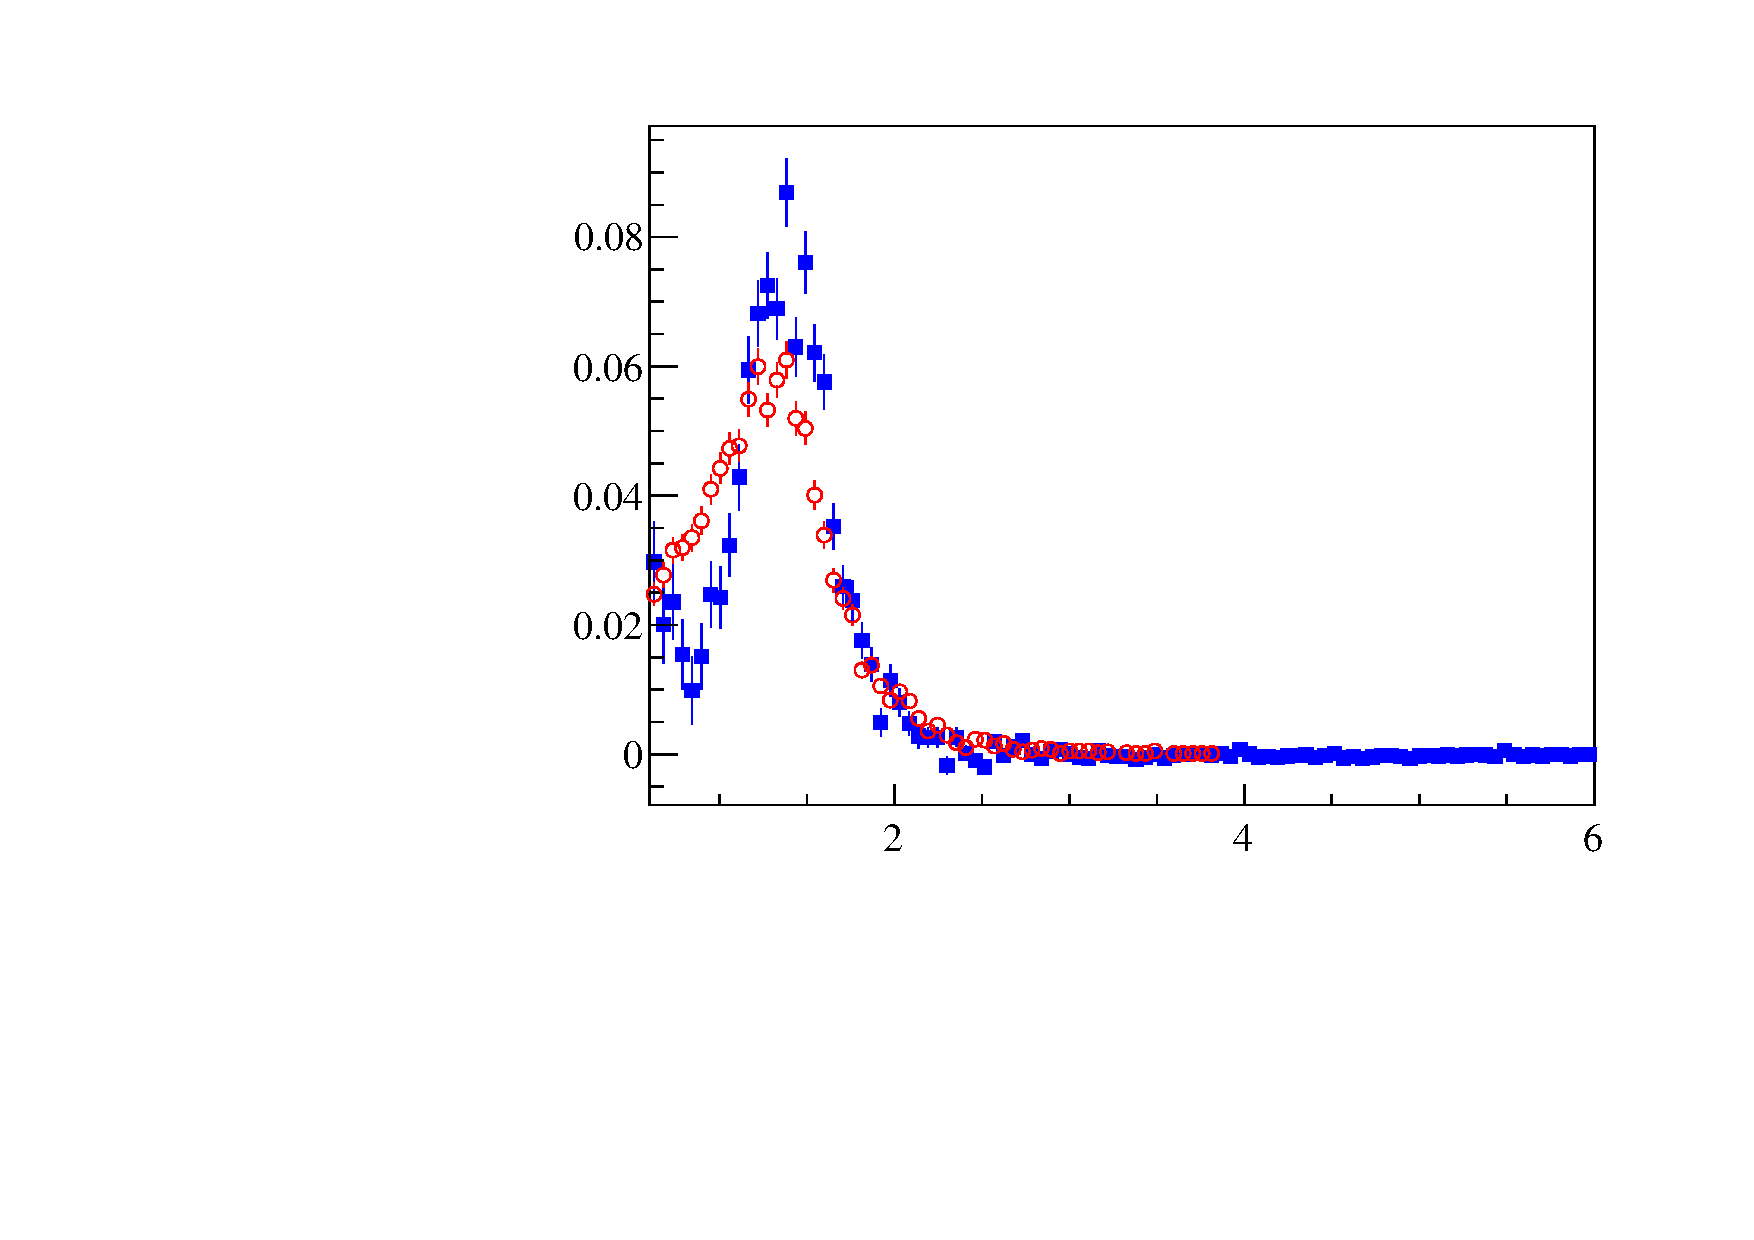
\includegraphics[width=50mm, height=35mm]{mc-data/pt_g_1p}
    }
    \put(50,0){
      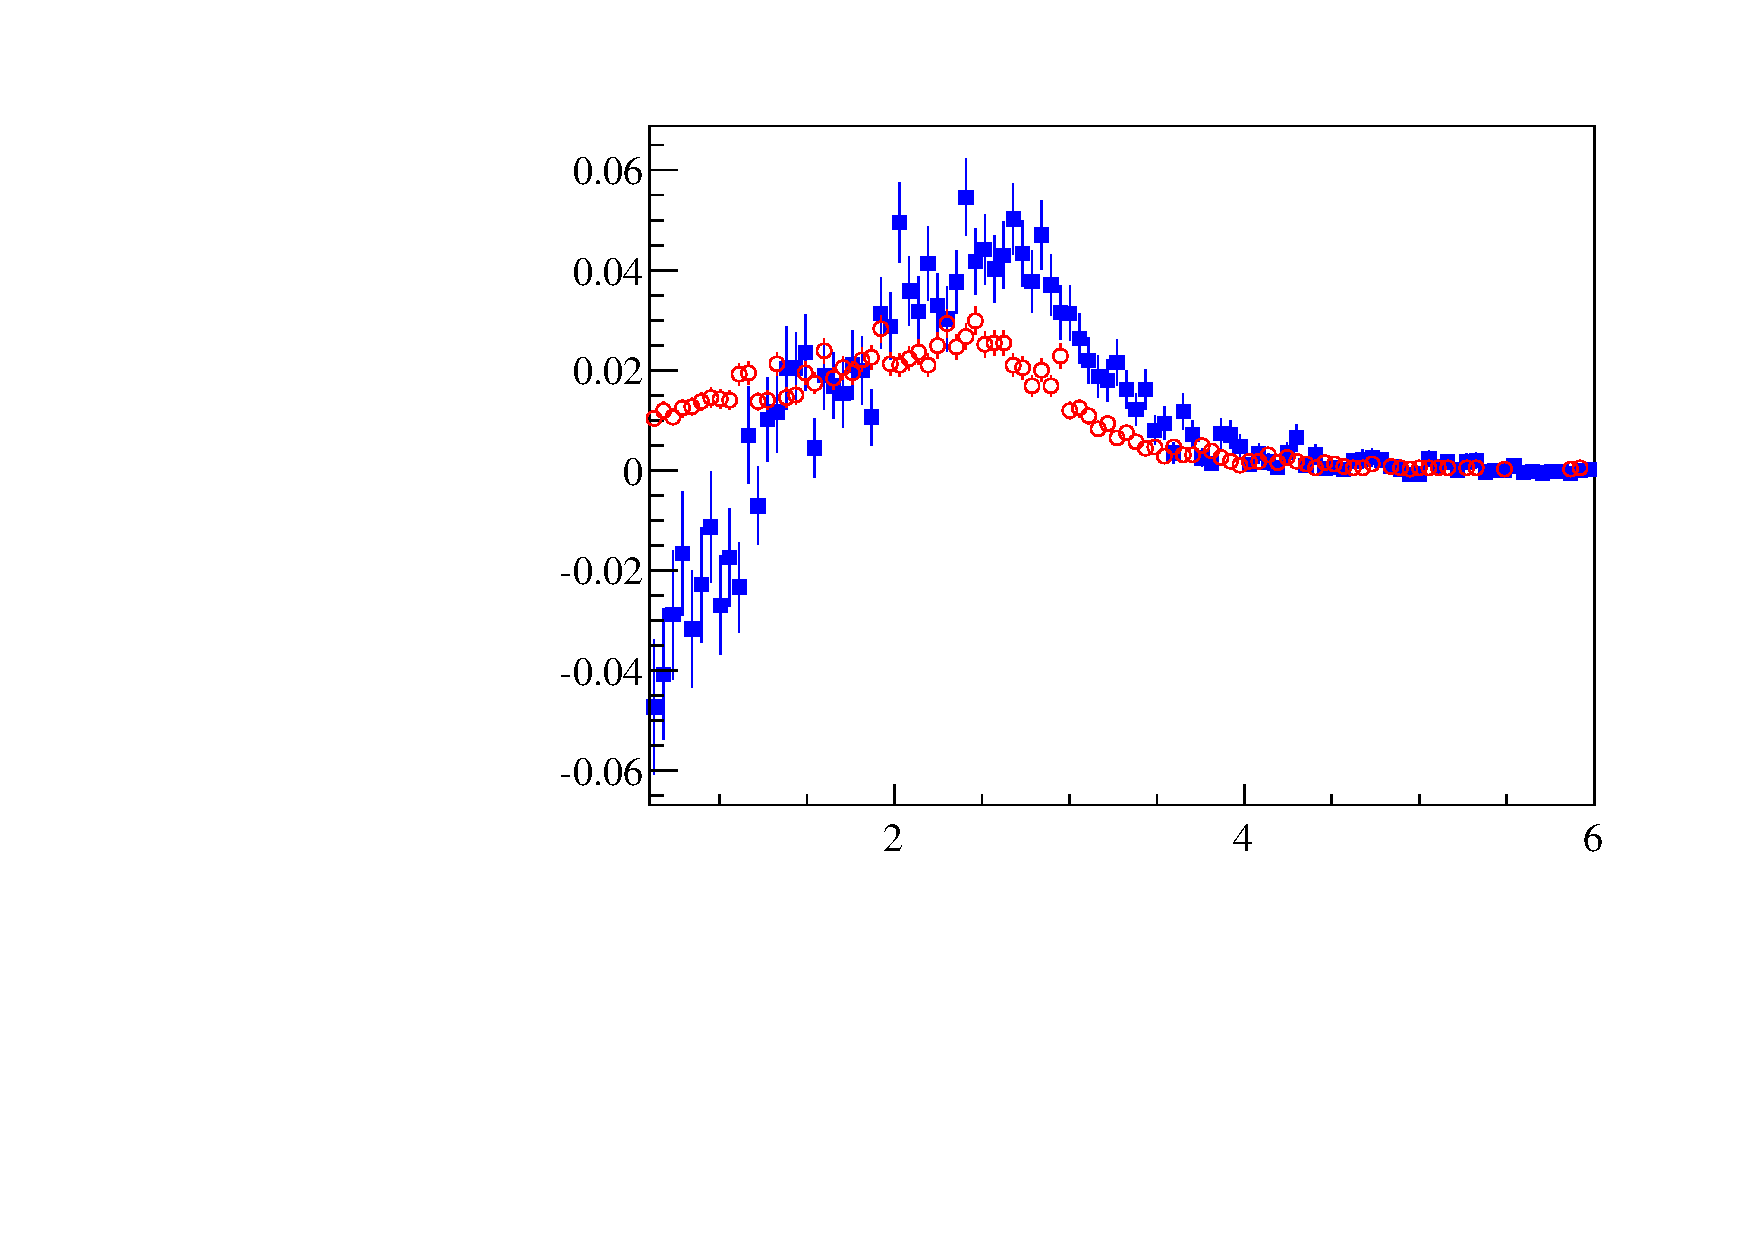
\includegraphics[width=50mm, height=35mm]{mc-data/pt_g_2p}
    }
    \put(100,0){
      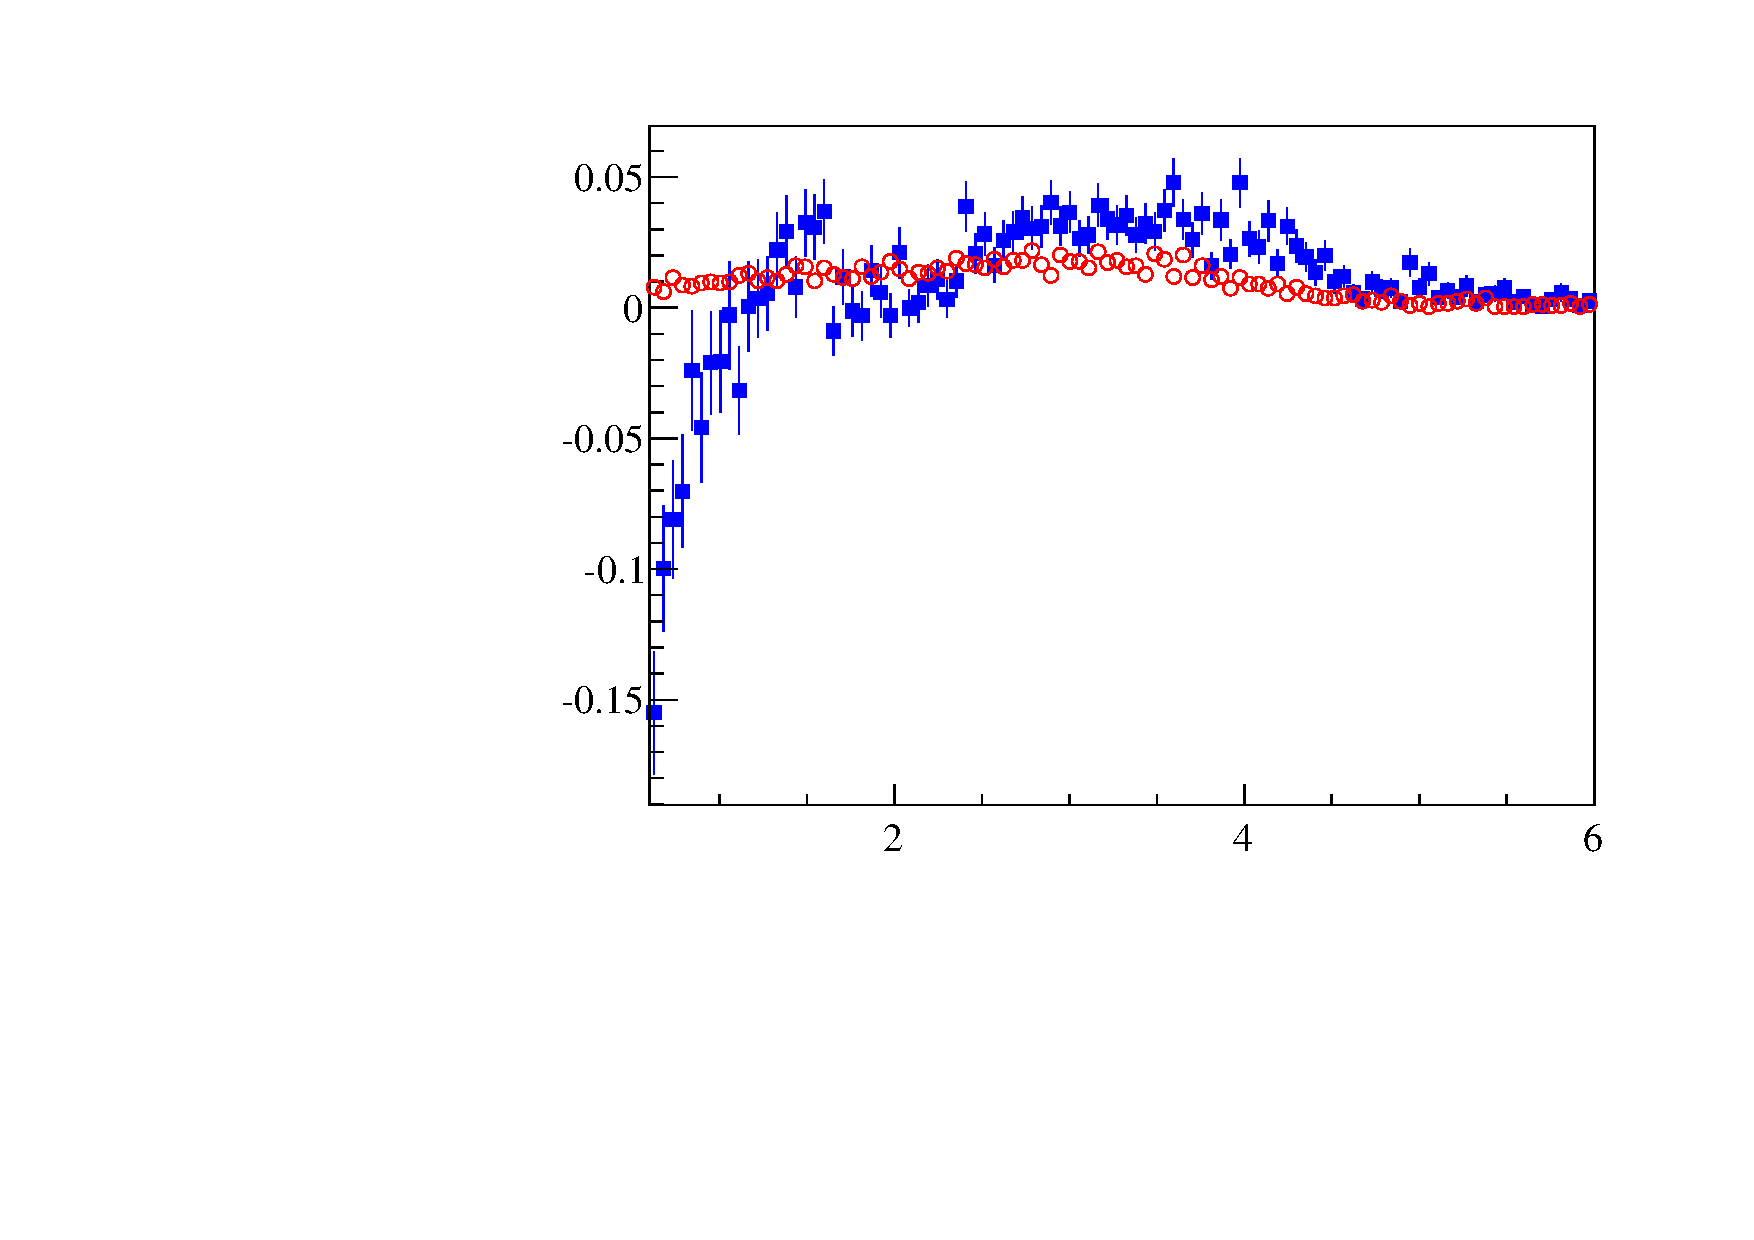
\includegraphics[width=50mm, height=35mm]{mc-data/pt_g_3p}
    }

    \put(15,-1){\scriptsize $p_T(\gamma) [\gevc]$ }
    \put(65,-1){\scriptsize $p_T(\gamma) [\gevc]$}
    \put(115,-1){\scriptsize $p_T(\gamma) [\gevc]$}

    \put(0,7){\scriptsize \begin{sideways}Arbitrary units\end{sideways}}
    \put(50,7){\scriptsize \begin{sideways}Arbitrary units\end{sideways}}
    \put(100,7){\scriptsize \begin{sideways}Arbitrary units\end{sideways}}

    \put(35,27){\scriptsize \chibOneP}
    \put(85,27){\scriptsize \chibTwoP}
    \put(135,27){\scriptsize \chibThreeP}
 
    % \graphpaper[5](0,0)(150, 175)        
  \end{picture}
}
\end{center}
\begin{alertblock}{}
This is due to the \sPlot\ technique, when applied on variables that affect the
background shape. In our study the background in the fit of the invariant mass
distribution depends on the photon transverse momentum, hence a mismatch
between data and simulation is expected.
\end{alertblock}

\end{frame}
